
\section{Расширения разнывной регрессии}

\begin{frame}{Расширения разнывной регрессии \footfullcite[Хороший обзор методов в][]{cattaneo2019extensions}}
\begin{enumerate}
    \item Кейс 1: что если у нас не одна отсечка, а несколько? Примеры:
    \begin{itemize}
        \item Округление непрывной $R$ в ценообразовании Uber
    \end{itemize}
    \item Что если у нас несколько running varables $R \in \mathbb{R}^2$
    \begin{itemize}
        \item Граница между территориями
        \item Избираются 3 кандидата, а не 2
    \end{itemize}
\end{enumerate}
    
\end{frame}

\begin{frame}{Пример: эффект территориальной газеты на явку \parencite{keele2015geographic}}
    \begin{figure}
        \centering
        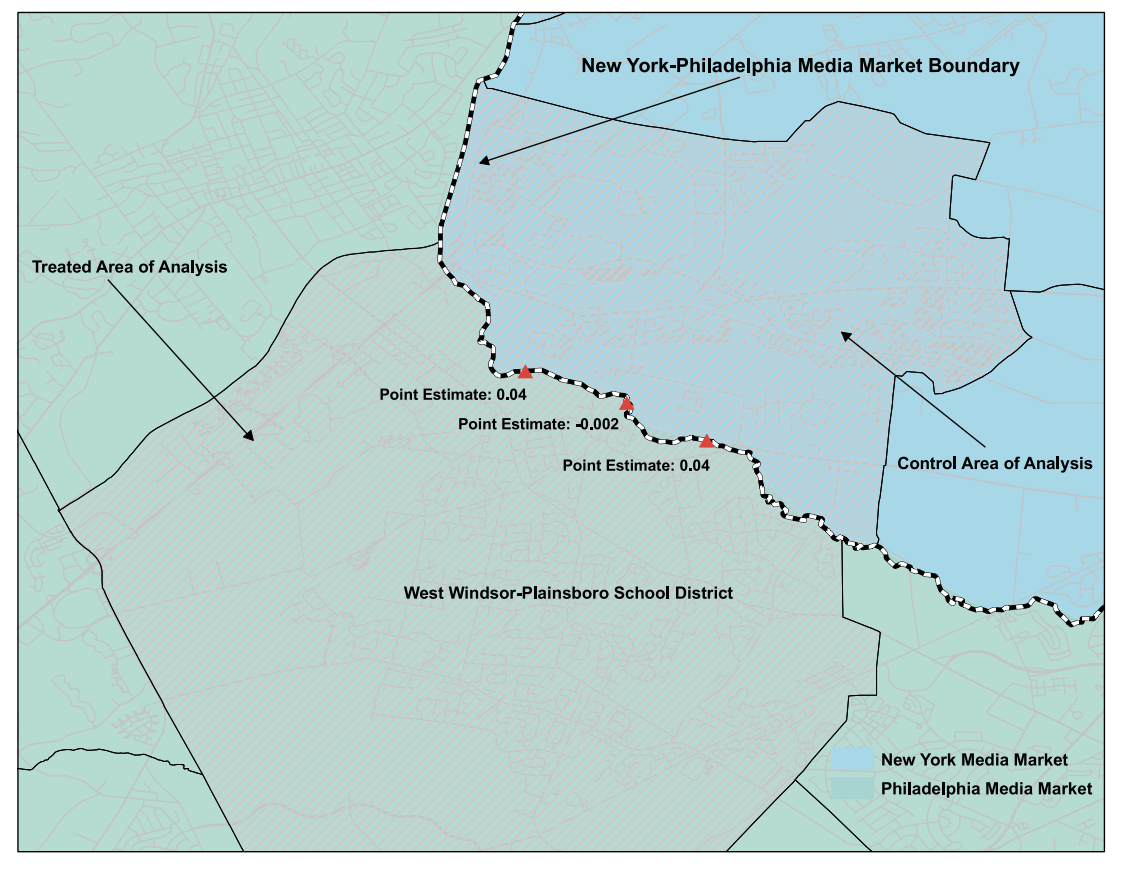
\includegraphics[width=\textwidth]{Images/geo.png}
    \end{figure}
\end{frame}


\begin{frame}{Возникает дисбаланс в ковариатах: интуиция \footcitetext[Картника и пример из ][]{keele2015geographic}}
    \begin{figure}
        \centering
        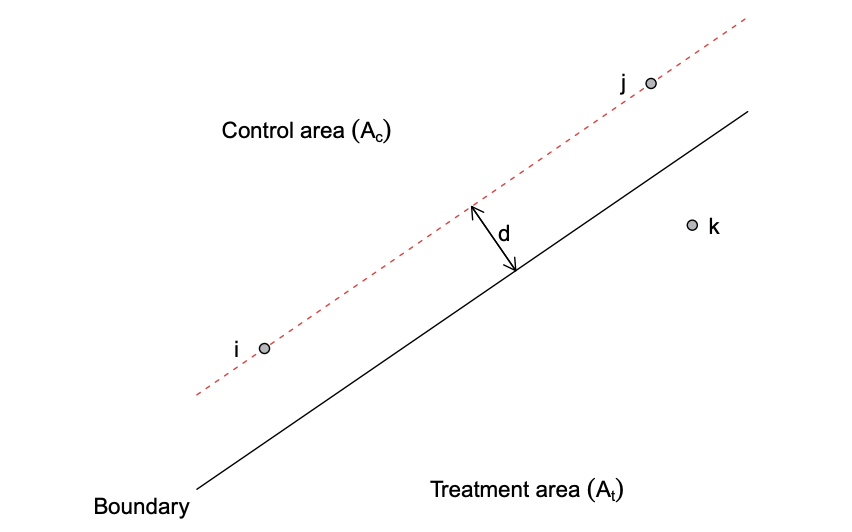
\includegraphics[width=\textwidth]{Images/pool bad.png}
    \end{figure}
\end{frame}


% \begin{frame}{Возникает дисбаланс}
%     \begin{figure}
%         \centering
%         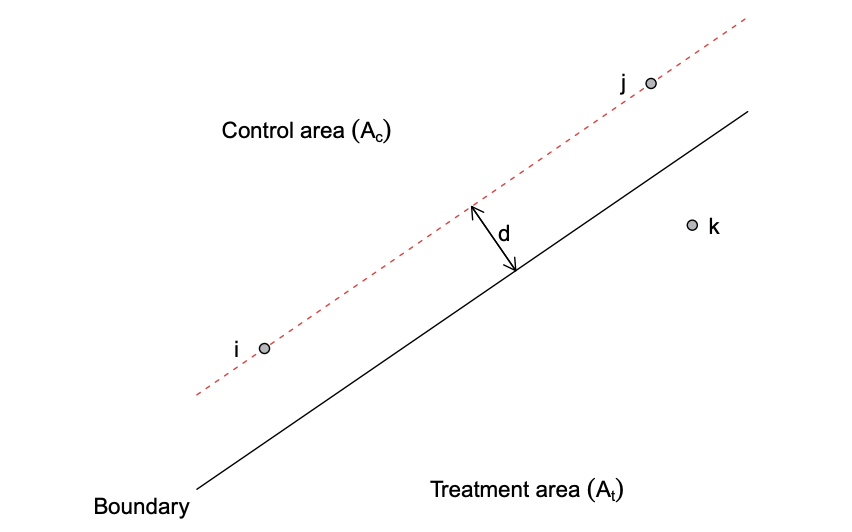
\includegraphics[width=\textwidth]{Images/pool bad.png}
%     \end{figure}
% \end{frame}
% теория, почему

\begin{frame}{Возникает дисбаланс в ковариатах: таблица}
    \begin{figure}
        \centering
        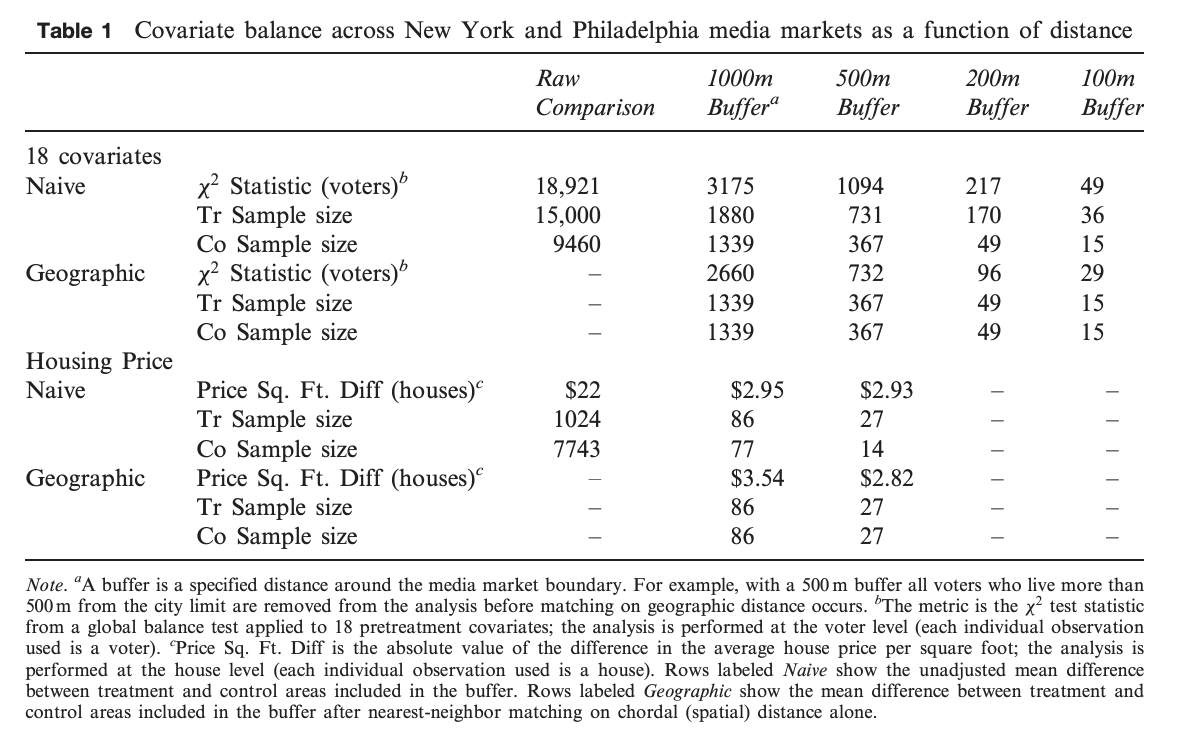
\includegraphics[width=\textwidth]{Images/geo_balance.png}
    \end{figure}
\end{frame}


\begin{frame}{Пример: эффект выбора 1 кандидата из 3 \parencite{cattaneo2016interpreting}}
    \begin{figure}
        \centering
        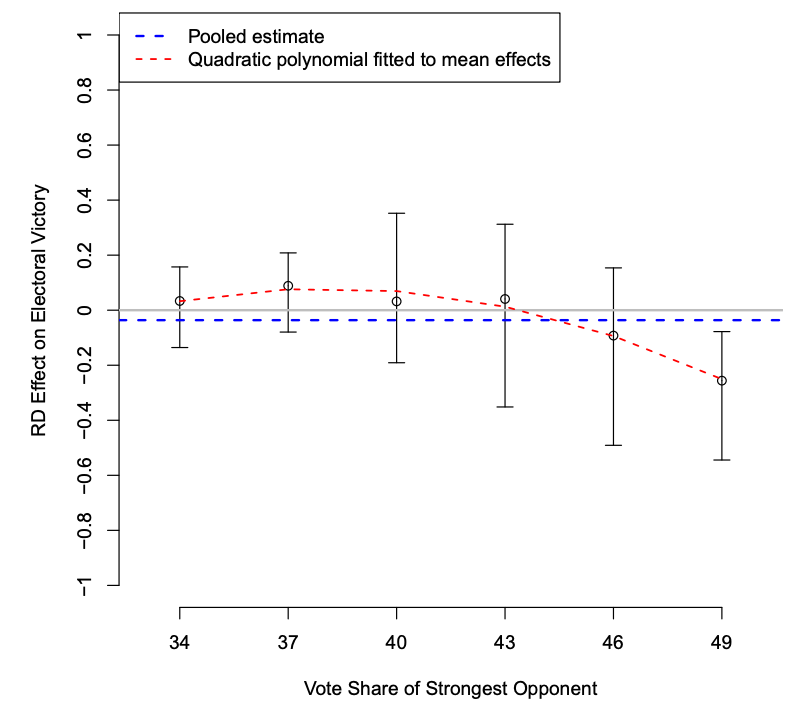
\includegraphics[width=0.8\textwidth]{Images/rdd_incumbancy_3.png}
    \end{figure}
\end{frame}



% https://scholar.google.com/scholar?hl=ru&as_sdt=0%2C5&q=regression+discontinuity+school+districts&btnG=

% R package https://arxiv.org/pdf/1912.07346.pdf

% Cattaneo book
% https://cattaneo.princeton.edu/books/Cattaneo-Idrobo-Titiunik_2018_CUP-Vol2.pdf
% https://arxiv.org/pdf/1911.09511.pdf


% robust ! ? 

% more interesting Extrapolating Treatment Effects in Multi-Cutoff Regression Discontinuity Designs

% https://ucu.edu.uy/sites/default/files/facultad/dcsp/RDcourse-Titiunik-Uruguay-Jul2016.pdf

% alternative cutoff values as falsification!

% need example here with a square zone

% another example differ across regions
% well, uber
